\documentclass[a4paper,11pt]{article}

% ---- inclusion of pictures
\usepackage[pdftex]{graphicx}

% ---- inclusion of code
\usepackage{listings}
\lstset{showstringspaces=false,frame=trBL,frameround=tttt,tabsize=4,basicstyle=\tiny,breaklines=true,breakatwhitespace=true}
\lstdefinestyle{bash}{language=bash}
\lstdefinestyle{Perl}{language=Perl}
\lstdefinestyle{C++}{language=C++}
\lstdefinestyle{DTD}{language=XML}
\lstdefinestyle{XML}{language=XML,usekeywordsintag=false,markfirstintag=true}
\newcommand{\includecode}[2]{\lstinputlisting[style=#1]{#2}}
\lstnewenvironment{code_bash}{\lstset{style=bash}}{}
\lstnewenvironment{code_perl}{\lstset{style=Perl}}{}
\lstnewenvironment{code_cpp}{\lstset{style=C++}}{}
\lstnewenvironment{code_dtd}{\lstset{style=DTD}}{}
\lstnewenvironment{code_xml}{\lstset{style=XML}}{}


\newcommand{\file}[1]{\texttt{#1}}
\newcommand{\cpp}[1]{\texttt{#1}}
\newcommand{\xml}[1]{\texttt{#1}}

%opening
\title{Commented Examples}
\author{
%Fran\c{c}ois Faure
}

\begin{document}

\maketitle

% \begin{abstract}
% 
% \end{abstract}

This document refers to examples located in directory \texttt{sofa/scenes/commentedExamples}.

\tableofcontents

\section{An oscillating particle}
Figure \ref{fig:massSpring} shows the mass-spring system we simulate.
\begin{figure}[ht]
	\centering
	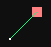
\includegraphics[width=0.4\linewidth]{massSpring01}
 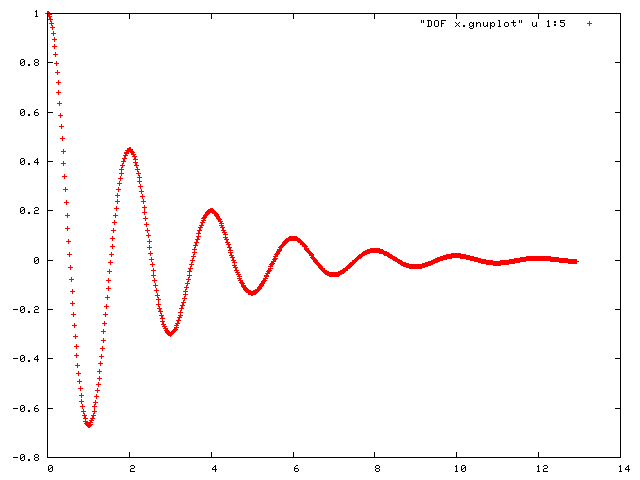
\includegraphics[height=0.4\linewidth]{euler_damped_ok}
	\caption{Left: white: moving particle, red: fixed particle, green: spring; Right: an x(t) trajectory.}
	\label{fig:massSpring}
\end{figure}

This scene is modeled for Sofa in \file{massSpring.scn} as:
\begin{code_xml}
<Node name="root" dt="0.02" showBehaviorModels="1" showForceFields="1">
   <Node name="mass-spring system">
      <Object type="MechanicalObject" name="DOF" position="0 0 0  1 0 0" velocity="0 0 0  0 1 0"/>
      <Object type="FixedConstraint" name="FixedConstraint" indices="0" />
      <Object type="UniformMass" name="totalMass" mass="1"/>
      <Object type="StiffSpringForceField" name="Spring" spring="0 1 10. 0. 1." />
      <Object type="Gravity" gravity="0.0 0.0 0.0"/>
      <Object type="Euler" symplectic="0"/>
   </Node>
</Node>
\end{code_xml}

The scene is structured using \emph{nodes} and \emph{objects}. Two nodes are used. 
The first, called \texttt{root}, represents the set of all simulation objects, which we call the \emph{scene}. 
The other node is called \texttt{mass-spring system}. 
It models our system.

A \emph{system} corresponds to a node. It is made of \emph{components}, called objects in the xml files, and sub-systems corresponding with children nodes.

Our system is described using six components, respectively:
\begin{itemize}
\item \emph{MechanicalObject} represents the degrees of freedom and their associated vectors. We have two particles at $0,0,0$ and $1,0,0$. The default velocities are null.
\item \emph{FixedConstraint} says that particle with index $0$ is fixed.
\item \emph{UniformMass} stores one single mass value for all the particles.
\item \emph{StiffSpringForceField} describes a list of springs, each of them modeled using index pair, stiffness, damping and rest length.
\item \emph{Gravity} says that the gravity is null.
\item \emph{Euler} says that the standard explicit Euler integration method should be applied. 
\end{itemize}
Notice that the scene description does not only describe the objects to simulate, but also the algorithms to apply.

This model is convenient because we can easily try variants.
We can of course modify the numerical parameters.
More importantly, we can replace one arbitrary component by another of the same kind, all the others remaining unchanged.
For example, we can replace \emph{Euler} by \emph{CGImplicit} to compare explicit and implicit time integration and to draw curves using the gnuplot export option.


Each node and object described in the xml file has an associated class in the Sofa library.
All the systems are implemented by the single \cpp{GNode} class, while the components are implemented using class hierarchies. 
The \emph{MechanicalObject} and the components which directly manipulate it are templated by \cpp{DataTypes} for code genericity.

\section{Livers} \label{sec:livers}
Figure~\ref{fig:liverTetra} shows the liver we simulate.
\begin{figure}[ht]
	\centering
	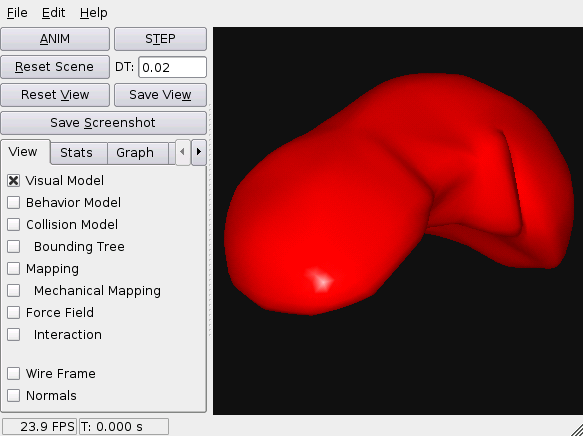
\includegraphics[height=0.3\linewidth]{liverTetra.png}
	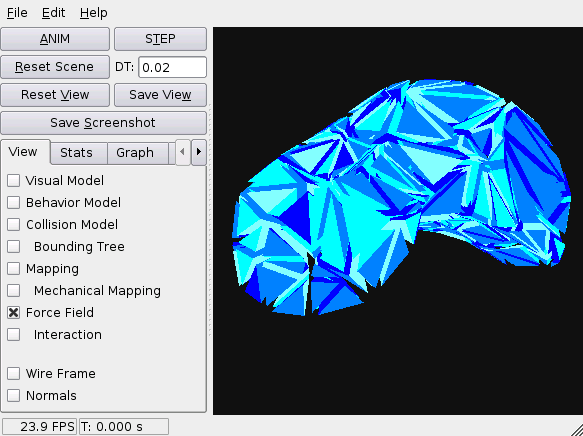
\includegraphics[height=0.3\linewidth]{liverTetra-force.png}
	\caption{Liver with tetrahedral FEM. Left: view of the visual model. Right: view of the force fields.}
	\label{fig:liverTetra}
\end{figure}

The model is described in file~\file{liverSpring.scn} as:
\begin{code_xml}
<Node name="root" dt="0.02" showBehaviorModels="0" showCollisionModels="0" showMappings="0" showForceFields="0">
	<Node name="Liver">
		<Object type="CGImplicit" iterations="25"/>
		<Object type="MechanicalObject" template="Vec3f" name="Liver" filename="BehaviorModels/liver.xs3"/>
		<Object type="DiagonalMass" name="mass" filename="BehaviorModels/liver.xs3"/>
		<Object type="Mesh" name="meshTopology" filename="Topology/liver.mesh"/>
		<Object type="TetrahedronFEMForceField" name="FEM" youngModulus="500" poissonRatio="0.3" computeGlobalMatrix="false" method="large"/>
                <Object type="FixedConstraint" name="FixedConstraint" indices="3 39 64" />
		<Node name="Visu">
			<Object type="OglModel" name="VisualModel" filename="VisualModels/liver-smooth.obj" color="red" />
			<Object type="BarycentricMapping" object1="../.." object2="VisualModel" />
		</Node>
	</Node>
</Node>
\end{code_xml}

The model has a \emph{Topology} and a \emph{TetrahedronFEMForceField}.
The first describes a topology a lists of elements such as edges, triangles, quads, tetrahedra. 
It is built on data given in auxiliary file.

The second uses the list of tetrahedra of the topology to apply tetrahedron-based FEM forces.

If desired, we can easily replace the TetrahedronFEMForceField with a set of springs based on the edges of the same tetrahedra.
We simply replace it by the following line, from file~\file{liverSpring.scn}:
\begin{code_xml}
<Object type="MeshSpringForceField" name="Springs" tetrasStiffness="400" tetrasDamping="4"/>
\end{code_xml}
The resulting model is shown in figure~\ref{fig:liverSpring}.
\begin{figure}[ht]
	\centering
	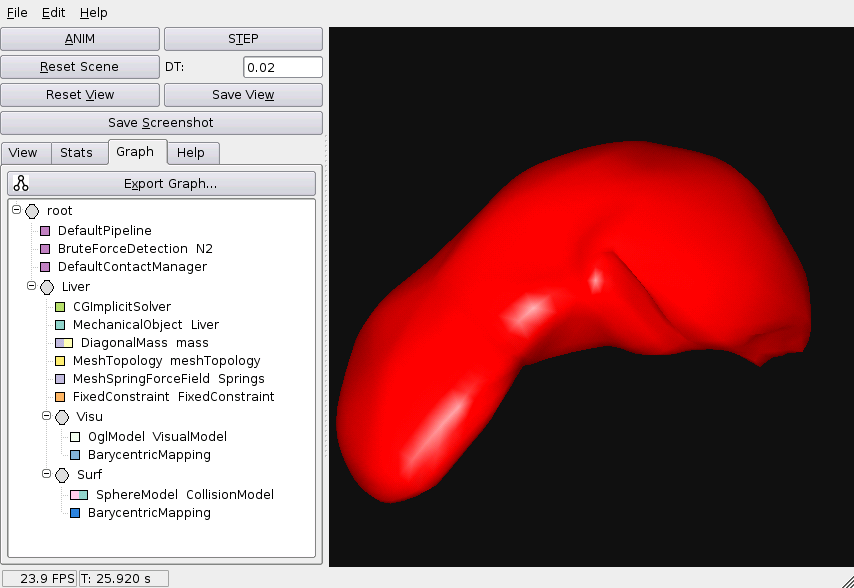
\includegraphics[height=0.3\linewidth]{liverSpring-graph.png}
	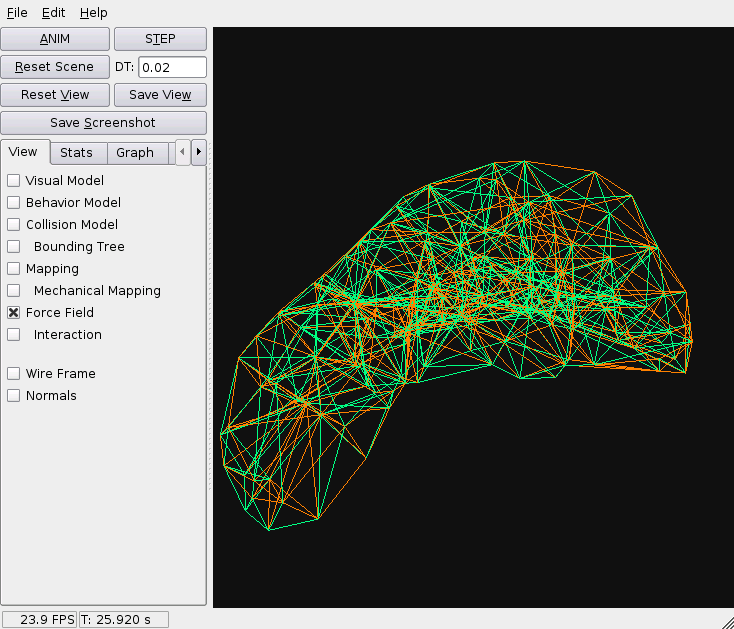
\includegraphics[height=0.3\linewidth]{liverSpring-force.png}
	\caption{The same model with tetrahedral FEM replaced by springs. Left: the scene graph. Right: the force field. }
	\label{fig:liverSpring}
\end{figure}






\section{An ffd-based liver model} \label{sec:ffd}
Figure~\ref{fig:ffd-lo} shows the model we simulate.
\begin{figure}[ht]
	\centering
	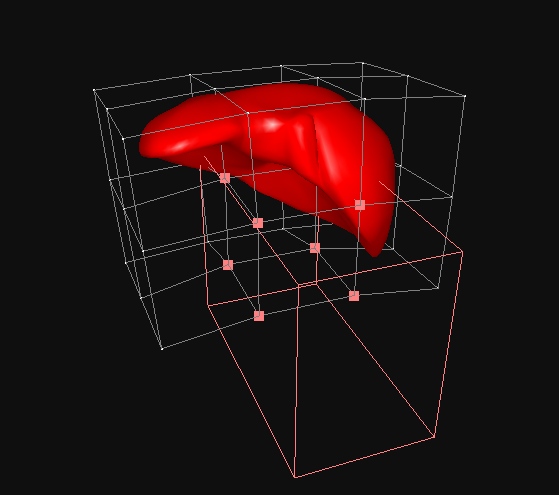
\includegraphics[height=0.3\linewidth]{ffd-lo}
	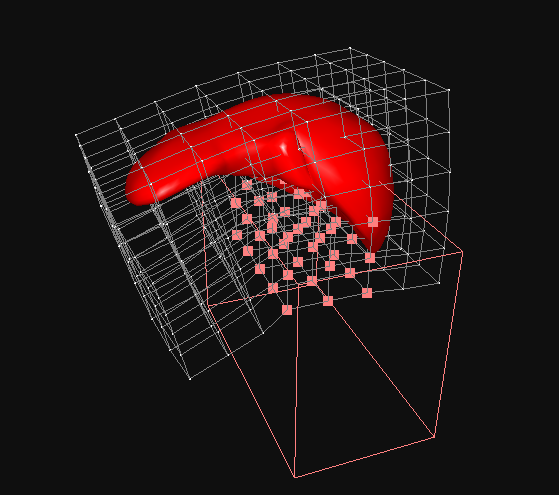
\includegraphics[height=0.3\linewidth]{ffd-hi} 
	\caption{The liver with a grid-based mechanical model at different resolutions. The pink points are fixed.}
	\label{fig:ffd-lo}
\end{figure}
The red surface is a visual model embedded in a deformable grid, whose corners are the independent degrees of freedom (DOF) of the system.
The pink box defines a volume where the DOF are constrained to remain fixed.
The DOF have associated mass and elastic forces.

The visual model is a geometry attached to the physical model. It is thus placed in a child node and attached using a \emph{BarycentricMapping}.
The topology and the initial vertex locations are first loaded form the given file. 
Then the barycentric coordinates of the vertices in the grid are computed and stored in the mapping.
During the simulation, the mapping updates the visual vertex locations based on the grid corners, acting as a Free Form Deformation (FFD) operator.


This scene is written in file \file{liverFFD.scn} as follows:
\begin{code_xml}
<Node name="root"  dt="0.04" showBehaviorModels="1" showMappings="0" showForceFields="1">
	<Node name="LiverFFD">
		<Object type="CGImplicit" symplectic="1"/>
		<Object type="MechanicalObject" />
		<Object type="UniformMass" mass="1.0" />
		<Object type="RegularGrid"
				nx="4" ny="3" nz="3"
				xmin="-5.25" xmax="2.25"
				ymin="0.25" ymax="5.25"
				zmin="-2" zmax="3"
			/>
		<Object name="GConstraint" type="BoxConstraint"
                        box="-3.5 -2 -5 0 3 2"
                        />
		<Object type="RegularGridSpringForceField" name="Springs" stiffness="160" damping="4" />
		<Node name="Visu">
			<Object type="OglModel" name="Visual" filename="VisualModels/liver-smooth.obj" color="red" />
			<Object type="BarycentricMapping" object1="../.." object2="Visual" />
		</Node>
	</Node>
</Node>
\end{code_xml}

The mapping from the grid corners to the vertices of the visual model is illustrated in figure~\ref{fig:ffd-map}.
\begin{figure}[ht]
	\centering
	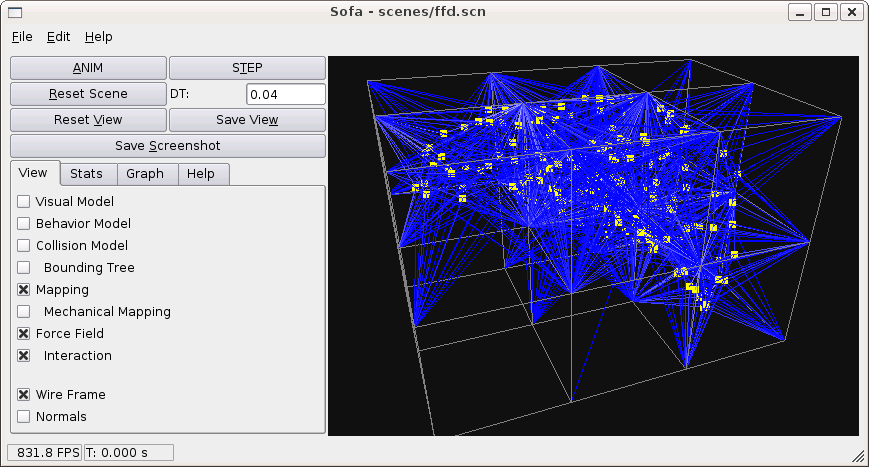
\includegraphics[width=0.8\linewidth]{ffd-map}
	\caption{The mapping (blue lines) form the corners of the deformable grid to the vertices of the visual model (yellow), visualized using the appropriate view options.}
	\label{fig:ffd-map}
\end{figure}

\section{Interactive manipulation}
\label{sec:interactive}
We want to interactively pick and pull points of the liver. To do this, we have to attach a \emph{CollisionModel} to the liver, as illustrated in figure~\ref{fig:collisionModel}.
\begin{figure}[ht]
	\centering
	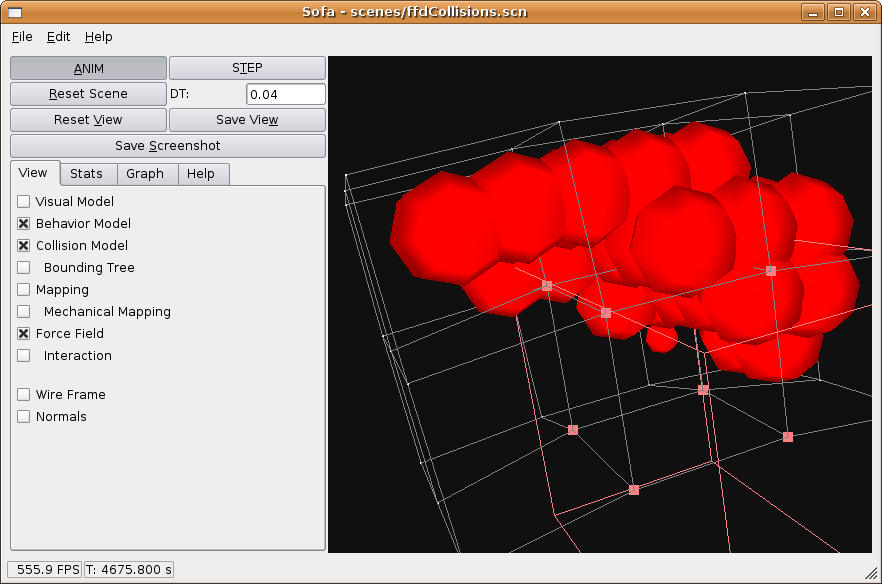
\includegraphics[width=0.48\linewidth]{collisionModel.png}
	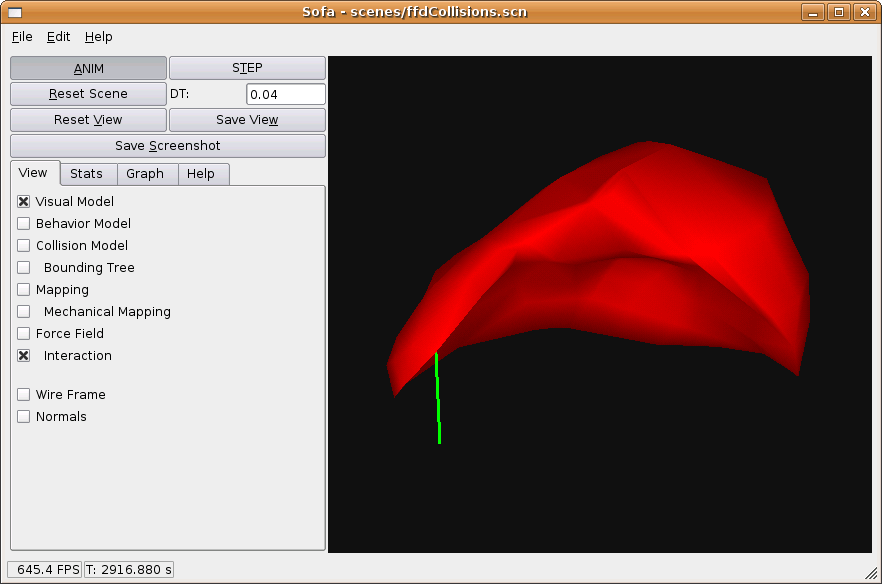
\includegraphics[width=0.48\linewidth]{collisionModel01.png}
	\caption{Left: a \emph{CollisionModel} made of spheres attached to the liver. Right: user interaction.}
	\label{fig:collisionModel}
\end{figure}
When shift-clicking in the graphics window, a ray is cast from the mouse pointer through the scene, and if it intersects with a collision surface, a spring between is created. This allows to interactively manipulate the model.

The scene is modeled in file \file{liverFFDCollisions.scn}:
\begin{code_xml}
<Node name="root"  dt="0.04" showBehaviorModels="1" showMappings="0" showForceFields="1">
  <Object type="CollisionPipeline" verbose="0" />
  <Object type="BruteForceDetection" name="N2" />
  <Object type="CollisionResponse" response="default" />
	<Node name="LiverFFD">
		<Object type="CGImplicit" symplectic="1"/>
		<Object type="MechanicalObject" />
		<Object type="UniformMass" mass="1.0" />
                <Object type="RegularGrid"
                        nx="8" ny="6" nz="6"
                        xmin="-5.25" xmax="2.25"
                        ymin="0.25" ymax="5.25"
                        zmin="-2" zmax="3"
                        />
		<Object name="GConstraint" type="BoxConstraint"
                        box="-3.5 -2 -5 0 3 2"
                        />
		<Object type="RegularGridSpringForceField" name="Springs" stiffness="160" damping="4" />
		<Node name="Visu">
			<Object type="OglModel" name="Visual" filename="VisualModels/liver-smooth.obj" color="red" />
			<Object type="BarycentricMapping" object1="../.." object2="Visual" />
		</Node>
                <Node name="Collision Surface">
                  <Object type="Sphere" name="Surf" filename="CollisionModels/liver.sph" />
                  <Object type="BarycentricMapping" />
                </Node>
	</Node>
</Node>
\end{code_xml}

There are two differences between this code and the version in section~\ref{sec:ffd}: a child node named \xml{Collision SUrface} has been added to node \xml{liverFFD}, and four objects related to collision detection and response have been added to node \xml{root}.

The collision model is defined in node \xml{Collision Surface} using two objects. Object \xml{Surf} describes the positions, velocities and radii of the collision spheres. Their values are read from file \file{liver.sph} at initialization time, and then attached to the independent DOF using a \emph{BarycentricMapping}. This mapping not only propagates positions and velocities bottom-up but also propagates forces top-down. This allows forces applied to the spheres to act on the independent DOF.

Direct interaction is set up by detecting the intersection of a pointer-based ray and the collision model. A spring between the ray is then created, and exists until the user releases the mouse button. This is achieved by the four objects added to the root node.

\end{document}
